% !TeX root = ../../main.tex
\section{Detailed reactor modelling: Toluene nitration (R101)}

\begin{wraptable}{r}{0.5\linewidth}
\centering
\caption{Reactor overview}
\label{tab:reactoroverview}
\begin{tabular}{@{}lS[table-format=4.2e1]s@{}}
    \toprule
    Parameter                    & {Value} & {Unit}         \\ \midrule
    Overall volumetric flowrate  & 1.32e-4 & \cubic\m\per\s \\
    Number of tubes              & 19      &                \\
    Diameter of each channel     & 0.2     & \m             \\
    Area of each channel         & 3.14e-2 & \square\m      \\
    Length of reactor            & 3.97    & \m             \\
    Aspect ratio                 & 19.8    &                \\
    Bed voidage                  & 0.39    &                \\
    Particle diameter            & 2e-4    & \m             \\
    Mass of H-mordenite required & 277     & \kg            \\
    Mass of inert SiC            & 4215    & \kg            \\
    Volume of liquid in reactor  & 9.24e-1 & \cubic\m       \\
    Total reactor volume         & 2.37    & \cubic\m       \\
    Total pressure drop          & 1.41e-1 & \bar           \\ \bottomrule
\end{tabular}
\end{wraptable}

The nitration of toluene in the heat exchanger reactor (R101) was chosen to be designed in detail for a few reasons. Firstly, the nitration process is most commonly carried out in batch or semi-batch reactors in industry \cite{dugal_nitrobenzene_2005}. Even though there have been incidents of nitration plant explosions such as the Xiangshui plant explosion, the industry has been slow in addressing these safety issues. As part of Nitroma's efforts to enhance the safety of the nitration process by transitioning from batch to continuous process, designing the nitration reactor in detail will allow Nitroma to develop a novel continuous reactor that is inherently safer. Moreover, the nitration reaction is a highly exothermic reaction, so the reactor needs to be robust in controlling the temperature to prevent thermal runaway. The reactor can be optimised to balance safety needs as well as efficient reaction performance. 

Additionally, the industrial nitration reaction typically uses sulfuric acid to protonate the nitric acid to form nitronium ions that are the main nitrating species \cite{sreedhar_scientific_2013}. However, the use of sulfuric acid is not environmentally-friendly as energy is needed to separate the products from the acid and further treatment needs to be done before discharging the sulfuric acid as a wastestream. Therefore, a detailed design of the nitration reactor will allow Nitroma to explore solid catalysts as a substitute, which will be key to Nitroma's goal of being a green company.  

\subsection{Reactor choices}
The reactor choices were considered based on several selection criteria, namely,
\begin{enumerate}
    \item Attrition of catalyst
    \item Hot spot formation
    \item Pressure drop
    \item Heat transfer
    \item Mass transfer
    \item Industrial scalability
\end{enumerate}

\begin{table}[H]
\begin{tabular}{@{}lll@{}}
\toprule
\textbf{Reactor Candidates}                 & \textbf{Pros}                                                                                               & \textbf{Cons}                                                                                    \\ \midrule
Stirred slurry reactor    & \begin{tabular}[c]{@{}l@{}}High degree of automation\\ especially temperature control\end{tabular} & High attrition of catalyst                                                              \\
Conventional packed-bed reactor    & Ease of operation and fast reaction                                                                & \begin{tabular}[c]{@{}l@{}}Flow maldistribution and \\ hot spots formation\end{tabular} \\
Microchannel packed bed reactor    & High heat and mass transfer rate                                                                   & High pressure drop (\textgreater{}40 bar)                                               \\
Coated wall microreactor           & Low pressure drop                                                                                  & Lack of industrial scalability                                                          \\
Plate heat exchanger reactor (HEX) & High heat transfer coefficient                                                                     & \begin{tabular}[c]{@{}l@{}}Challenging catalyst\\ regeneration process\end{tabular}     \\
Shell-and-tube HEX                 & \begin{tabular}[c]{@{}l@{}}Low pressure drop and\\ high heat transfer coefficient\end{tabular}     &                                                                                         \\ \bottomrule
\end{tabular}
\end{table}

What were the selection criteria, what other alternatives were considered and why were they ruled out? 
selection criteria: - attrition of catalyst
- 
%Thinking of creating a table of saying reactor choices//why cannot choose this reactor//
Several reactors for this reaction were considered for this nitration process including  
The choice of reactors was discussed in detail in \cref{sec:reactorchoices}.

\subsection{Heat of reaction}
To understand the thermal effects of the reaction, the enthalpy of reaction was initially calculated using the enthalpy of formation for each compound participating in the reaction. Data on the standard heat of formation for the compounds were sourced from the NIST website and literature papers. A full table of the source of each enthalpy can be found in [link to appendix/ supporting info]. 

The enthalpy of reaction was calculated using Hess Law, as shown in the equation below:
\begin{equation}
  \Delta H_{r}^{T} = \Delta H_{f,\mathrm{nitrotoluene}}^{T} + \Delta H_{f,\mathrm{water}}^{T} - \Delta H_{f,\mathrm{toluene}}^{T} - \Delta H_{f,\mathrm{nitric acid}}^{T}
\end{equation}

Since the reaction was carried out at 330K, the enthalpy of reaction was adjusted to the operating temperature by using the heat capacities of the compounds using the equation below. The enthalpy of reaction was not further adjusted to capture the effects of pressure because pressure has a negligible effect on the overall enthalpy [liu, 2019]. 

\begin{equation}
  \Delta H_{r}^{330K} = \Delta H_{r}^{\standardstate} + C_p \Delta T
\end{equation}

P-nitrotoluene is an exception since it is a solid at standard state. Therefore, the latent heat of fusion needs to be included when adjusting the enthalpy of reaction to the operating temperature. The summary of the enthalpy of formation for all reactants and products can be found in Appendix \ref{tab:Heat enthalpy table}. The final enthalpy of reaction at 330K is calculated to be -116 kJ/mol. At the specified flowrates of the reactants, the heat duty of the reactor is -63.4 kW.

\subsection{Axial dispersion}
\label{sec:axialdispersion}

\begin{wrapfigure}{r}{0pt}
    \vspace{-\intextsep}
    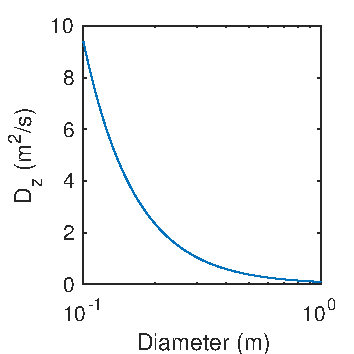
\includegraphics[scale=0.8]{figures/D_z}
    \caption{Dispersion}
    \label{fig:dispersion}
\end{wrapfigure}
The axial dispersion was calculated as it is an important parameter in affecting the performance and conversion of the packed-bed reactor. 

The axial dispersion coefficient ($D_z$) can be calculated using the Taylor expression: 
\begin{equation}
    D_z=D_{ab}+\frac{(uD)^2}{192D_{ab}}
    \label{axial dispersion coefficient}
\end{equation}
The values of $D_{ab}$ was calculated using the Wilke-Chang correlation.
\begin{equation}
    D_{ab}=\frac{7.4\cdot 10^{-8}(\phi M_2)^{0.5}T}{\mu V_1^{0.6}}
    \label{wilkechang}
\end{equation}
where $D_z$ is the axial dispersion model, $D_{ab}$ is the diffusion coefficient $u$ is the superficial velocity, $\phi$ is the association parameter which is estimated to be 1 for toluene, $M_2$ is the molecular weight of the solvent which is calculated based on the volumetric ratio of nitric acid and water, $V_1$ is the molar volume of toluene at boiling point.
The axial dispersion coefficient ($D_z$) was calculated to for various diameters and plotted based on \cref{axial dispersion coefficient,wilkechang}.

From \cref{fig:dispersion}, it can be observed that the dispersion coefficient decreases sharply after after ~10cm. Thus, a diameter of 23cm has been selected as any further increase in the diameter does not warrant the drawback of the increasing pressure drop ($\Delta P$), as the $d_p$ is inversely proportional to $\Delta P$ based on \cref{eqn:ergun}.


\subsection{Adiabatic temperature}

\textcolor{red}{Include adiabatic temp rise with and without cooling water}

The nitration reactor cannot be assumed to be isothermal because nitration is a highly exothermic process. As seen in Fig. [adibatic], the temperature rises sharply in the first xxx meters before plateauing at xxx K for an adiabatic reactor. Even by cooling the reactor with a cooling jacket, the exit temperature remains at xxx. The temperature of the reaction needs to kept below 140 °C. At temperatures higher than that, thermal decomposition of nitric acid occurs, which releases nitrogen dioxide and produces even more heat, leading to thermal runaway. Other $NOx$ emission safety risks have been covered in section \ref{sec:NOx}. Additionally, the possibility of hotspot as shown in Fig [hotspot] will speed up the deactivation of catalyst, but more importantly, it poses safety concerns through the risk of thermal runaway [ref]. Therefore, to maintain the safety of the plant, the temperature of the reactor needs to be well-controlled.

\begin{figure}[h]
    \centering
    
    \begin{subfigure}{0.32\linewidth}
        % 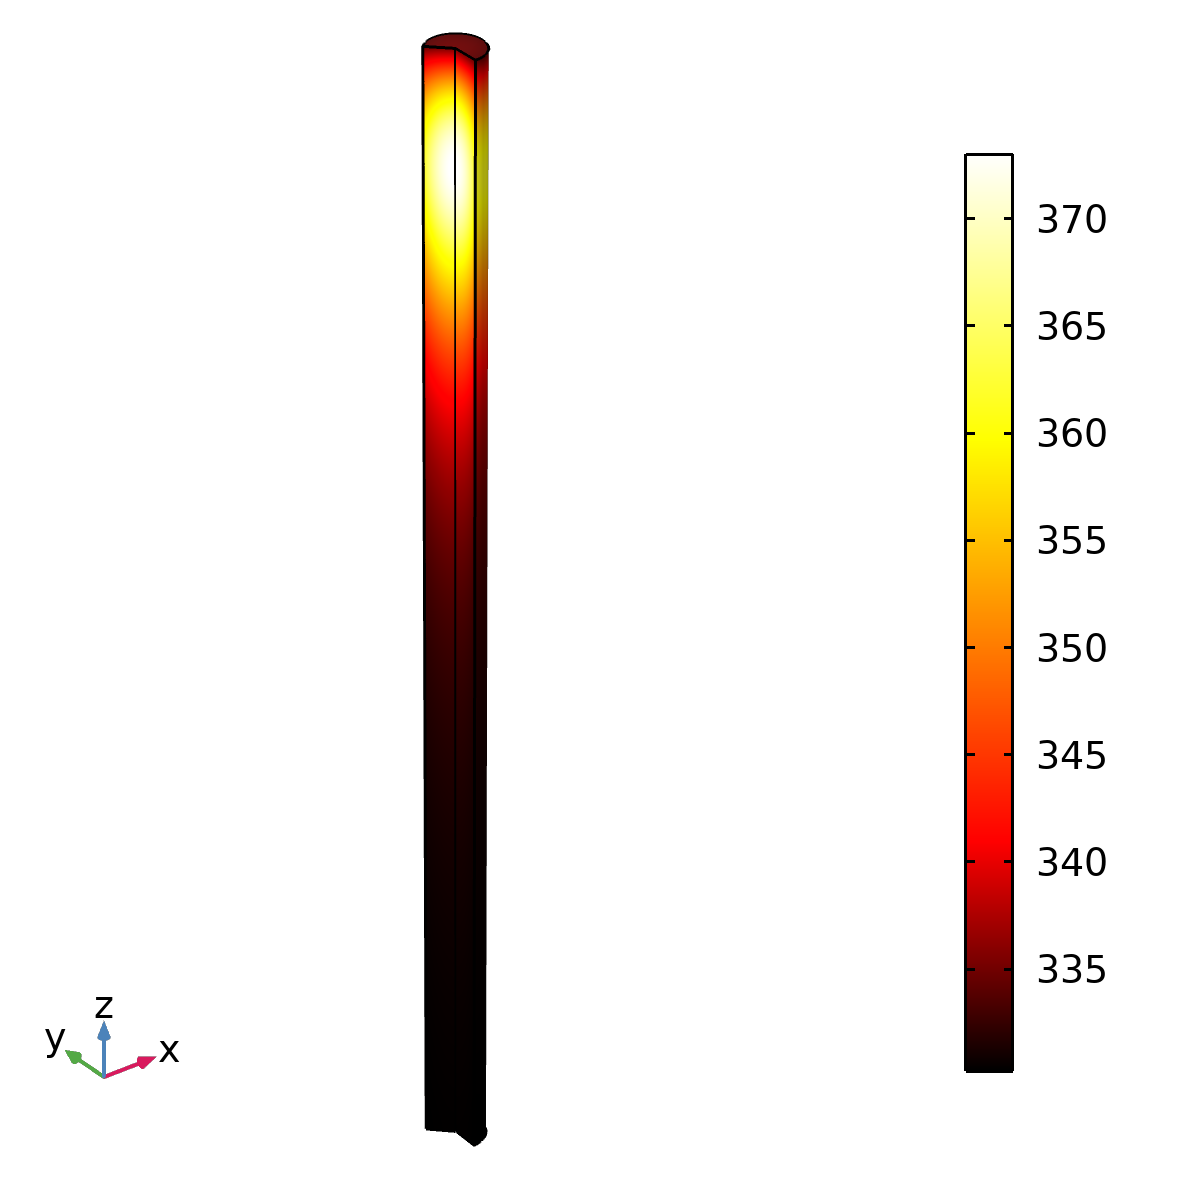
\includegraphics[width=\linewidth]{figures/simple-tube-temperature.png}
        \caption{Adiabatic reactor temperature}
    \end{subfigure}
    \begin{subfigure}{0.32\linewidth}
        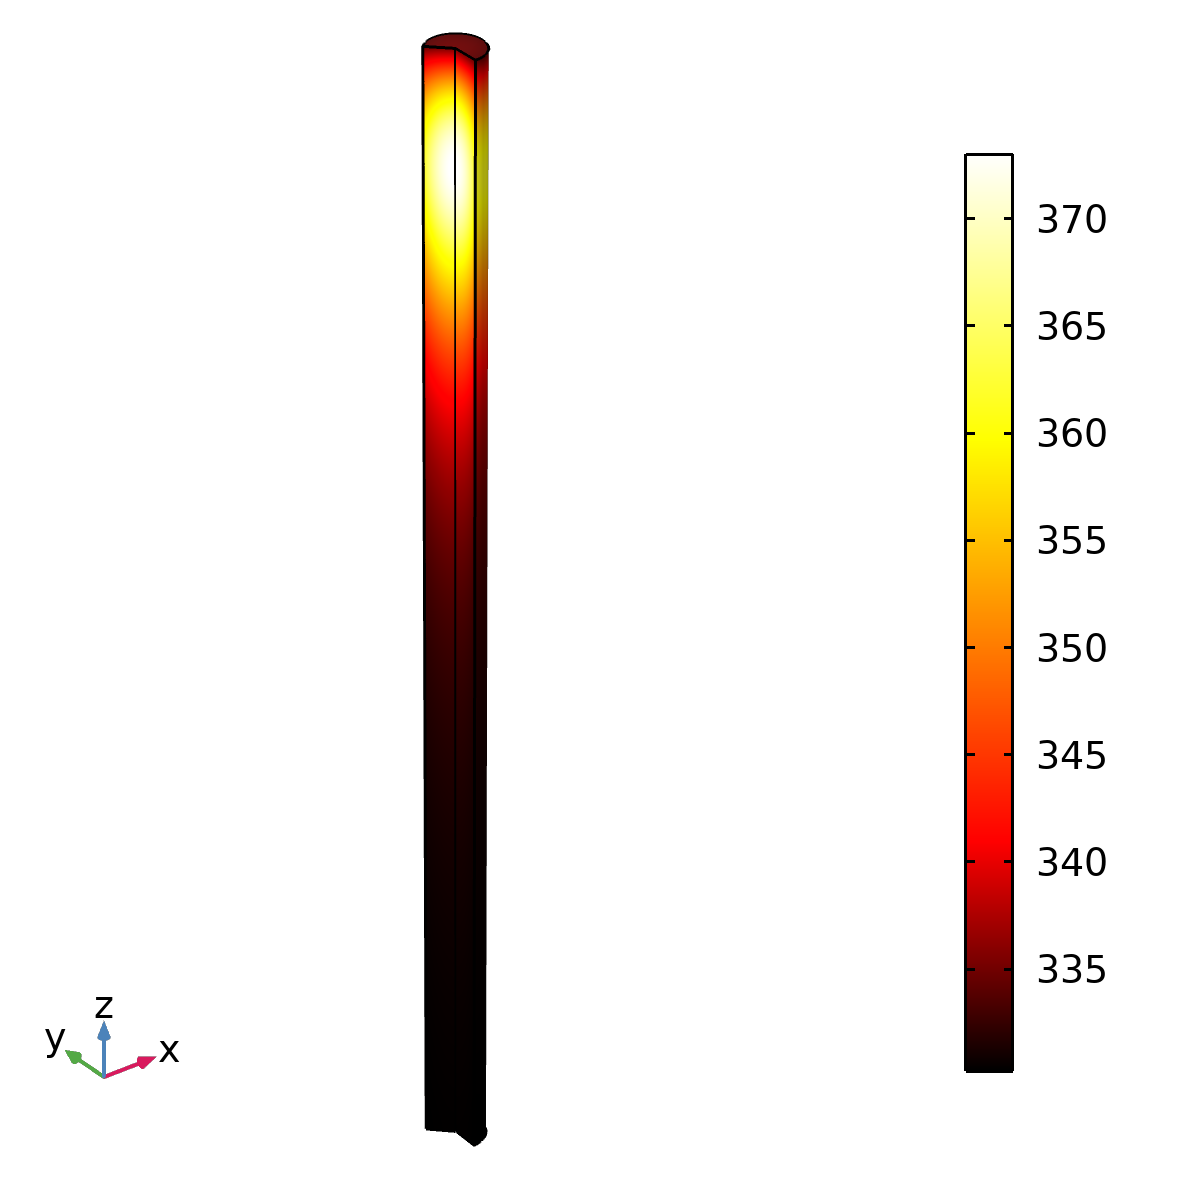
\includegraphics[width=\linewidth]{figures/simple-tube-temperature.png}
        \caption{Temperature with external cooling}
    \end{subfigure}
    \begin{subfigure}{0.32\linewidth}
        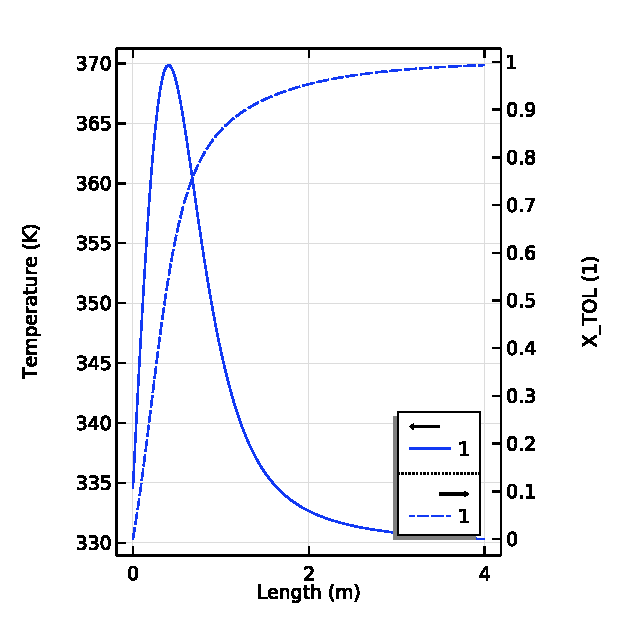
\includegraphics[width=\linewidth]{figures/simple-tube-T-X.eps}
        \caption{Temperature and conversion profiles}
    \end{subfigure}

    \caption{Temperature profiles for adiabatic reactor, and with external cooling}
    \label{fig:simple-tube}
\end{figure}

\subsection{Catalyst specification}
\subsubsection{Catalyst support}
Silicon Carbide (SiC) was chosen as the catalyst support owing to its high thermal conductivity (83 W m \textsuperscript{-1} K \textsuperscript{-1} as compared to 3 W m \textsuperscript{-1} K \textsuperscript{-1} for H-mordenite [ref]). This helps to lower the overall temperature in the reactor by reducing the catalyst surface temperature [ref]. Although as a result, the rate of reaction and conversion are relatively lower, using SiC keeps the temperature below the critical temperature before thermal runaway happens. 

Besides, an important feature of the SiC catalyst support is that the tortuosity of the structure promotes homogeneous mixing of the reactants, much like a static mixer [ref]. As the nitration of toluene is a two-phase reaction, the well-mixed flow increases the interphase contact area, and subsequently increases the rate of reaction. Thus, the reaction can be modelled as a single phase reaction. [can be moved to other sections] 

Additionally, the nitration reactor would require 270 kg of H-mordenite catalyst to achieve the desired rate and conversion. However, this could lead to collapse of the catalyst bed due to its weight, which could lead to significant attrition of catalyst and severe pressure drop [ref]. The mechanical strength of the SiC support will ensure the catalyst is strongly kept in place when fluid flows through it. The strength of the SiC catalyst support does not decrease over time because SiC forms a silica film when in contact with HNO3 solution, therefore rendering it passive against corrosion [ref]. The strength and durability of SiC makes it an ideal material as a catalyst support. The SiC catalyst support used will be fabricated using the partial sintering process with 30 \% porosity before coating it with H-mordenite catalyst.

\subsubsection{Catalyst size}
The H-Mordenite catalyst used in the nitration reaction is deposited on the SiC foam by washcoating. Since the nitration reaction takes place on the surface of the catalyst, it is important to reduce the effect of external and internal diffusional limitation of the reaction depending on the size of the catalyst particle.  

The catalyst particle size was chosen to be 2 µm. At this particle size, the effectiveness factor of the catalyst is $\approx$ 1. An effectiveness factor of $\approx$ 1 suggests that external and internal mass transfer resistances of the catalyst are negligible and the actual rate of reaction is not lowered by mass transfer resistances. The diffusional limitations within the catalyst can also be assumed to be negligible, since the Weisz-Prater criterion of the chosen catalyst size is $\ll$ 1. Detailed calculation of these calculation can be found in Appendix xxx.

Typically, catalyst grains, pellets and beads of this diameter would result in a huge pressure drop across the reactor. However, due to the open structure of SiC foam, the pressure drop is significantly reduced [duong viet et al]. In fact, with the same surface area per volume of catalyst bed, catalyst supports have a pressure drop over 10 times smaller than the corresponding packed bed [richardson et al]. The small catalyst size used in the reaction can therefore reap the benefits of negligible diffusional limitations while avoiding any significant pressure drop.

\subsection{Pressure drop}
%The pressure drop of is a significant consideration in during the selection and modelling of this reactor as the packed-bed reactor shows the 
Even though the pressure drop is expected to be insignificant, efforts were taken to verify the pressure drop of the reactor.

The pressure drop in this was calculated by using the modified Ergun equation from [lacroix et al]: 
\begin{equation}
    \frac{\Delta p}{L} = \frac{150 \mu (1- \varepsilon)^2 u_0}{\varepsilon^3 d_p^2} + \frac{1.75(1-\varepsilon)\rho u_0^2}{\varepsilon^3 d_p}
    \label{eqn:ergun}
\end{equation}
where foam porosity ($\varepsilon$) is 0.30 from [Byung-KoogJang et al], $d_p$ is the particle diameter equivalent to the SiC foam structure based only on its mean window size ($a$), using the following formula:
\begin{equation}
d_{p}=\frac{3a[(4 / 3 \pi)(1-\varepsilon)]^{1 / 2}}{2(1-[(4 / 3 \pi)(1-\varepsilon)]^{1 / 2})}
\end{equation}

The pressure drop was calculated to be 0.33 bar which poses no safety risk to the plant. No high pressure pumps will be required, thus saving both OPEX and CAPEX costs.

A final number of tubes ($n_t$) of 7 was chosen based on the centered hexagonal number rule (\cref{eqn: hexagon} which has practical usage in industry for maximising tube bundles into large cylindrical containers. 
\begin{equation}
    n^3 - (n-1)^3 = 3n(n-1)+1
    \label{eqn: hexagon}
\end{equation},
where $n$ represents the sequence of hexagonal number. 

From plot Y, it can be observed that a final number of tubes ($n_t$) of 7 in the multitubular packed-bed reactor will provide a required length ($L$) of \textcolor{red}{4.2m}, and allowing an acceptable pressure drop ($\Delta P$)of \textcolor{red}{0.1bar}.

\subsection{Novel triple concentric tubes}
\label{sec:tripleconctube}
[needs to be expand further]
Triple concentric tubes heat exchanger (TCTHE) was considered to allow for better temperature control in the reactor. It increases the heat transfer rate through the larger heat exchange area between the fluid and both the inner and outer side of the annulus \cite{moya-rico_characterization_2019}. An enhanced heat exchange network within the reactor maintains the temperature in the desirable temperature range of < 90°C for the reaction, which will be detailed in Section [xxx]. Furthermore, a higher heat transfer rate per unit length from the reaction to the cooling fluid in the TCTHE reduces the overall size of the reactor, therefore leading to space and cost savings. The cooling water used in the nitration reactor will be reused from xxx reactor at xxx K to maximise the energy recovery in Nitroma's plant. 

